\chapter{算法介绍}
\section{引言}
本文基本的研究思路是使用数值模拟算法和深度学习算法来研究流变学本构方程建模的问题。本文第一部分基于动态时序建模理论,构建门控循环单元网络(GRU)的预测模型,通过深度学习算法处理数值模拟生成的时变本构关系数据,重点解析循环神经网络在时间序列建模中的特征提取机制,主要涉及的算法有GRU算法,本章同时综述了时间序列数据的其他深度学习算法。第二部分引入物理约束的智能建模策略,针对实际流变实验数据构建融合物理信息的混合神经网络模型,重点整合了物理信息神经网络(PINN)的微分方程嵌入技术、基于注意力机制驱动的多源特征融合方法,以及结合条件变分自编码框架(CVAE)的生成式建模策略,实现物理规律约束下的数据-模型双驱动建模。

本章将在此基础上,对研究中所涉及的关键算法进行理论概述,并阐述算法选型的依据,以系统性地综述相关领域的研究进展,为后续研究奠定理论基础。
\section{算法介绍}
\subsection{时间序列数据介绍}
时间序列数据是指在一系列时间点上按时间顺序排列的数据点集合。这些数据点通常是连续或定期记录的,反映了某个变量随时间的变化情况。在流变学研究中,时间域的应力应变数据在小应变时满足玻尔兹曼叠加原理,即当前应力状态为之前所有应变历史的线性和\cite{boltzmannZurTheorieElastischen1878}。大应变时应力应变数据虽然不满足玻尔兹曼的线性叠加,但是依旧可以表示为过去应变历史的非线性关系叠加。

\subsection{循环神经网络}
\subsubsection{简单RNN}
循环神经网络(Recurrent Neural Network,RNN)是一种专门处理序列数据的神经网络结构,其核心在于利用循环结构捕捉时间或顺序上的依赖关系\cite{elmanFindingStructureTime1990}。RNN的基本结构由输入层、隐藏层和输出层组成(图\ref{rnn_gru illustration}(a))。隐藏层中的神经元不仅接收来自输入层的信号,还接收来自前一时刻隐藏层的信号。这种循环连接使得RNN能够捕获序列中的时间依赖关系。
RNN的数学模型可以通过公式\eqref{eq:rnnht}描述:
\begin{align}
   & \mathbf{h}_t = \sigma(\mathbf{W}_{xh} \mathbf{x}_t + \mathbf{W}_{hh} \mathbf{h}_{t-1} + \mathbf{b}_h) \label{eq:rnnht} \\
   & {\mathbf{o}_t = \mathbf{W}_{ho} \mathbf{h}_t + \mathbf{b}_o} \label{eq:rnnot}
\end{align}
其中$\mathbf{h}_t$ 是时刻 $t$ 的隐藏状态,$\mathbf{x}_t$ 是时刻 $t$ 的输入,$\mathbf{o}_t$ 是时刻 $t$ 的输出,$\mathbf{W}_{xh}$ 是输入到隐藏层的权重矩阵,$\mathbf{W}_{hh}$ 是隐藏层到隐藏层的权重矩阵,$\mathbf{W}_{ho}$ 是隐藏层到输出层的权重矩阵,$\mathbf{b}_h$ 和 $\mathbf{b}_o$ 是偏置。$\sigma$是激活函数,通常使用 $\tanh$ 或 $\text{ReLU}$。RNN 的训练过程通常使用反向传播算法。通过计算梯度来更新权重矩阵,从而最小化损失函数。

在简单的RNN中,存在梯度消失问题,这主要源于反向传播过程中梯度的连乘效应\cite{schmidhuber1997long}。损失函数 $L$ 对 $\mathbf{W}_{hh}$ 的梯度可以表示为公式\eqref{eq:rnngradient}:
\begin{align}
  \frac{\partial L}{\partial \mathbf{W}_{hh}} = \sum_{t=1}^{T} \frac{\partial L}{\partial \mathbf{h}_t} \cdot \frac{\partial \mathbf{h}_t}{\partial \mathbf{W}_{hh}} \label{eq:rnngradient}
\end{align}
展开后,隐藏状态关于$\mathbf{W}_{hh}$ 的导数为公式\eqref{eq:rnngradient2}:
\begin{align}
  \frac{\partial \mathbf{h}_t}{\partial \mathbf{W}_{hh}} = \sigma'(\mathbf{W}_{hh} \mathbf{h}_{t-1} + \mathbf{W}_{xh} \mathbf{x}_t + \mathbf{b}_h) \cdot \mathbf{h}_{t-1}^T \label{eq:rnngradient2}
\end{align}
注意到,$\frac{\partial L}{\partial \mathbf{h}_t}$依赖于前一个时间步的梯度,如公式\eqref{eq:rnngradient3}:
\begin{align}
  \frac{\partial L}{\partial \mathbf{h}_t} = \frac{\partial L}{\partial \mathbf{h}_{t+1}} \cdot \frac{\partial \mathbf{h}_{t+1}}{\partial \mathbf{h}_t} = \frac{\partial L}{\partial \mathbf{h}_{t+1}} \cdot \mathbf{W}_{hh} \cdot \sigma'(\mathbf{h}_t) \label{eq:rnngradient3}
\end{align}
这表明梯度在通过时间反向传播时会乘以$\mathbf{W}_{hh}$。
从时间$t$到时间$T$的梯度可以表示为公式\eqref{eq:rnngradient4}:
\begin{align}
  \frac{\partial L}{\partial \mathbf{h}_t} = \left( \prod_{k=t+1}^{T} \mathbf{W}_{hh} \cdot \sigma'(\mathbf{h}_{k-1}) \right) \cdot \frac{\partial L}{\partial \mathbf{h}_T} \label{eq:rnngradient4}
\end{align}
其中乘积 $\prod_{k=t+1}^{T} \mathbf{W}_{hh} \cdot \sigma'(\mathbf{h}_{k-1})$在某些情况下可能会非常小,例如如果 $\mathbf{W}_{hh}$的特征值小于1,那么随着$(T - t)$的增加,$\mathbf{W}_{hh}^{T-t}$将呈指数级减小并趋近于零。
如果反向传播过程中每一项都小于1,那么整个乘积将随着 $(T - t)$的增加呈指数级减小。
这意味着对于远离输出端的时间步$t$,梯度$\frac{\partial L}{\partial \mathbf{h}_t}$将非常小,导致权重更新几乎停止,这就是RNN的梯度消失问题。由于RNN为了捕捉时间依赖性,我们不可避免地设置长时间步,这导致RNN梯度消失问题几乎难以避免。
\subsubsection{GRU}
为了解决简单RNN的梯度消失问题,Schmidhuber等提出了长短期记忆网络(Long Short-Term Memory,LSTM)\cite{schmidhuber1997long}。LSTM通过引入门控机制来控制信息的流动,从而有效地缓解梯度消失问题。LSTM的核心结构包括输入门、遗忘门和输出门,这些门控机制能够有效地控制信息的流动,从而捕获长期依赖关系。

LSTM虽然通过引入门控机制有效地解决了简单RNN中的梯度消失问题,但在实际应用中仍然存在一些问题。LSTM包含三个门(输入门、遗忘门、输出门),导致其参数数量较多,增加了模型的复杂度和计算成本。由于LSTM的复杂结构,其训练和推理速度相对较慢,尤其是在处理大规模数据时。为了解决LSTM的上述问题,Cho等提出了GRU作为LSTM的简化版本\cite{choLearningPhraseRepresentations2014}(图\ref{rnn_gru illustration}(b))。GRU的设计初衷是为了简化LSTM的结构,同时保持其捕获长期依赖关系的能力。GRU只有重置门(Reset Gate)和更新门(Update Gate)两种门控单元,与LSTM相比,GRU的参数数量较少,训练和推理速度更快。重置门的计算公式为公式\eqref{eq:grureset}。
\begin{align}
  \mathbf{r}_t = \sigma(\mathbf{W}_r \mathbf{x}_t + \mathbf{U}_r \mathbf{h}_{t-1} + \mathbf{b}_r) \label{eq:grureset}
\end{align}
更新门的计算公式为公式\eqref{eq:gruupdate},重置门决定了前一时间步的隐藏状态在多大程度上被忽略。当重置门的输出接近0时,网络倾向于“忘记”前一时间步的信息,仅依赖于当前输入;而当输出接近1时,前一时间步的信息将被更多地保留。
更新门决定了多少过去的信息将被保留,而新信息将占据多少比例。当更新门的输出接近1时,新的隐藏状态几乎等同于旧的隐藏状态,从而实现了长期依赖的捕捉;当更新门的输出接近0时,新的隐藏状态将主要由当前输入决定。
\begin{figure}[htbp]
  \centering
  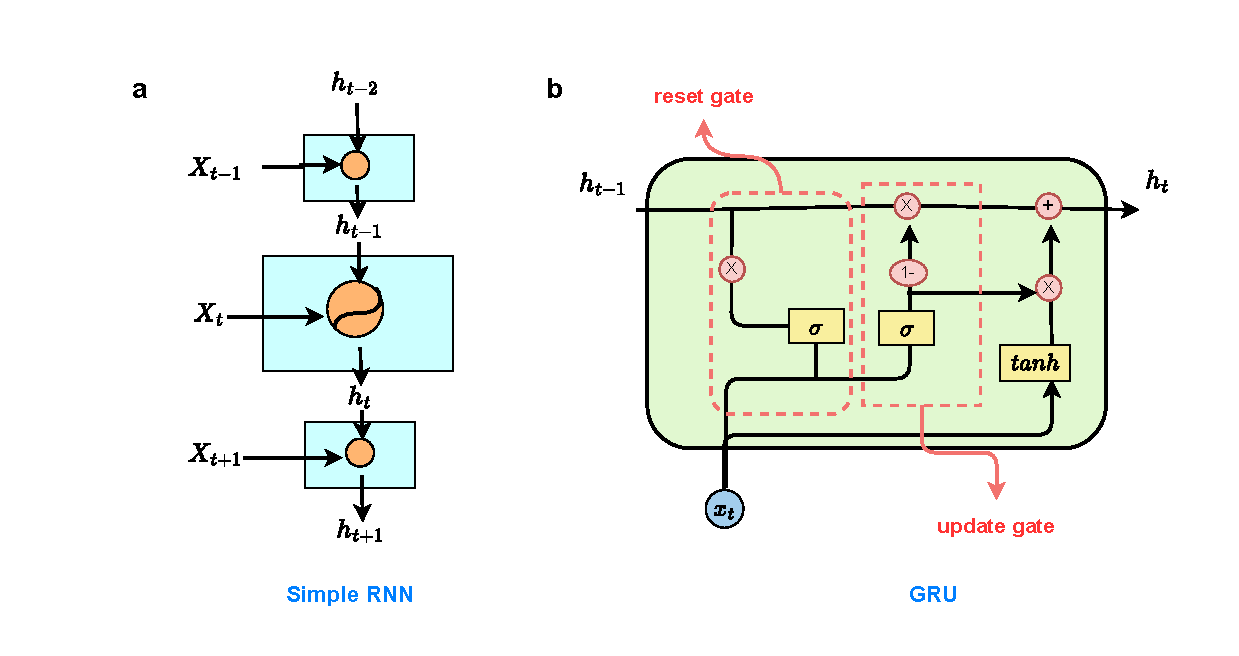
\includegraphics[width=0.9\textwidth]{Fig/rnn-gru.pdf}
  \FigureBicaption{\label{rnn_gru illustration}(a)RNN 示意图 ;(b)GRU 示意图}{Schematic illustration of (a) RNN and (b) GRU}
\end{figure}
\begin{align}
  \mathbf{z}_t = \sigma(\mathbf{W}_z \mathbf{x}_t + \mathbf{U}_z \mathbf{h}_{t-1} + \mathbf{b}_z) \label{eq:gruupdate}
\end{align}
候选隐藏状态决定了当前时间步的新信息,如公式\eqref{eq:gruhih}所示。
\begin{align}
  \tilde{\mathbf{h}}_t = \tanh(\mathbf{W}_h \mathbf{x}_t + \mathbf{U}_h (\mathbf{r}_t \odot \mathbf{h}_{t-1}) + \mathbf{b}_h) \label{eq:gruhih}
\end{align}
当前隐藏状态如公式\eqref{eq:gruhi}所示,这里的当前隐藏状态与上文LSTM的隐藏状态含义是一样的。
\begin{align}
  \mathbf{h}_t = (1 - \mathbf{z}_t) \odot \mathbf{h}_{t-1} + \mathbf{z}_t \odot \tilde{\mathbf{h}}_t \label{eq:gruhi}
\end{align}

GRU移除了单元状态的概念,直接从门控单元来计算隐藏状态,GRU 通过重置门和更新门的协同工作,实现了对信息流动的有效控制,使得网络能够在需要时记住长期依赖关系,同时减少梯度消失/爆炸的问题。GRU的结构比LSTM更简单,计算效率更高,因此在实践应用中广受欢迎。本章使用GRU模型进行流变学本构方程的预测建模。
\subsection{其他时间序列算法}
在深度学习领域,针对时间序列数据的处理方法已呈现出多样化的趋势。除了传统的循环神经网络(RNN)及其变体,近年来研究人员提出多种新型网络架构,包括卷积神经网络(CNN)、Transformer以及Mamba网络等,这些方法在时间序列分析中展现出显著的优势。

卷积神经网络(CNN)最初是为图像处理任务设计的,但其在时间序列分析中的应用也取得了显著成效\cite{lecun1998gradient}。通过引入一维卷积操作,CNN能够有效地从时间序列数据中提取局部特征。由于卷积操作具有权值共享的特性,CNN在处理长序列数据时表现出较高的计算效率,并且能够有效规避传统RNN中常见的梯度消失或梯度爆炸问题。通过多层卷积结构的堆叠,CNN能够捕获更为复杂的时间依赖性,进而在语音识别、金融预测等实际应用中表现出优异的性能\cite{li2021survey}。

Transformer模型是近年来在自然语言处理(NLP)领域取得突破性进展的架构,其核心在于自注意力机制(Self-Attention)\cite{Vaswanietal2017Attention}。与传统的RNN类模型不同,Transformer摒弃了序列顺序处理的限制,转而通过全局上下文信息建模序列中各元素之间的依赖关系。这种机制使得Transformer能够并行处理长序列数据,并捕获全局时序特征。在时间序列分析任务中,Transformer通过自注意力机制能够聚焦于序列中的关键时间点,从而有效建模时序依赖性和非线性关系。这一特性使其在机器翻译、语音识别等任务中超越了传统模型的表现。

Mamba网络是近年来提出的一种新型时间序列处理架构,专门针对复杂时间序列数据的高效建模而设计\cite{gu2024mamba}。与传统的RNN或CNN模型相比,Mamba网络通过引入多尺度时序建模策略,能够同时捕获时间序列中不同时间尺度的特征。这种多尺度建模方法不仅增强了模型的表达能力,还提升了其在处理多变且复杂时序数据时的鲁棒性。Mamba网络的独特之处在于其能够整合多层次时序信息进行联合建模,从而为不同时间粒度的变化提供更为精确的预测。这一特性使其在金融市场分析、气象预测等领域展现出广阔的应用前景。

这些方法不仅拓展了时间序列建模的理论边界,也为实际应用提供了更为强大的工具。本文的研究工作是选择一种可以处理时间序列的算法来对数值模拟的流变学数据进行建模预测,样本量在万级,属于中小规模数据集,综合考虑算法时空间复杂度和训练成本,选择RNN中的GRU作为算法模型。未来针对更多流变学数据和复杂场景,可以进一步研究其他前沿模型的应用。
\section{物理信息神经网络}
\subsection{理论基础}
物理信息神经网络(Physics-Informed Neural Networks, PINN)是一种结合深度学习和物理知识的神经网络模型,旨在通过数据驱动的方式求解偏微分方程(PDE)\cite{raissiPhysicsinformedNeuralNetworks2019a}。与传统数据驱动的神经网络模型相比,PINN在训练过程中引入了物理约束,使得模型不仅能够学习数据中的模式,还能够满足物理定律,从而提高模型的泛化能力和预测精度。PINN的基本思想是将物理定律(如偏微分方程)作为先验知识嵌入到神经网络中,通过最小化数据损失和物理损失来训练模型。这样,PINN不仅能够学习数据中的模式,还能够满足物理定律,从而提高模型的泛化能力和预测精度。在实际应用中,PINN可以通过损失函数强制模型满足物理约束,从而提高模型的物理合理性和可解释性。
\begin{figure}[htbp]
  \centering
  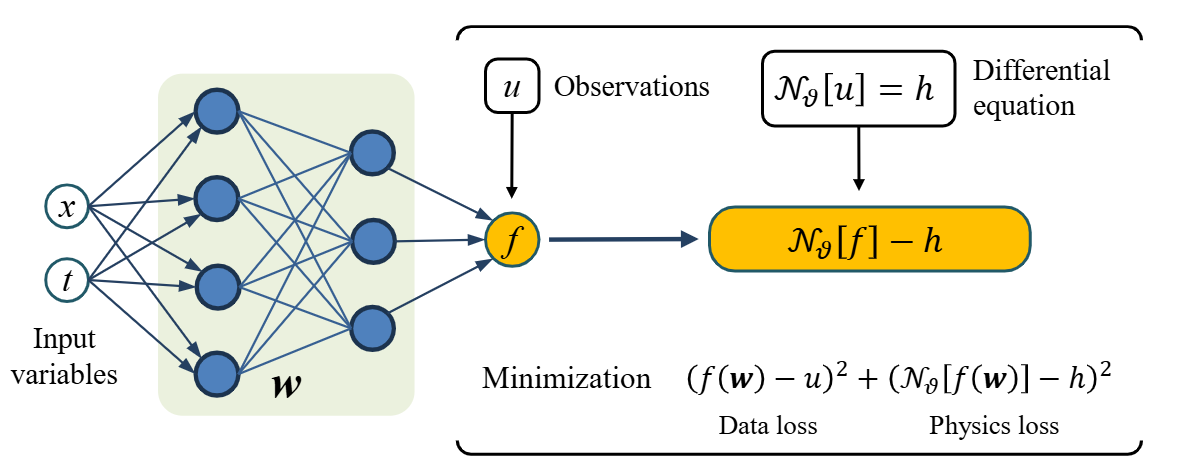
\includegraphics[width=0.8\textwidth]{Fig/pinn_logo.png}
  \FigureBicaption{\label{pinn illustration}PINN 示意图\cite{cuomoScientificMachineLearning2022}}{Schematic illustration of PINN\cite{cuomoScientificMachineLearning2022}}
\end{figure}
PINN的优势在于其能够通过物理方程进行训练,极大减少了对大量标注数据的需求。此外,PINN能够确保模型的预测符合实际的物理规律,从而避免了数据驱动模型可能出现的不合理结果。尽管PINN在处理复杂问题时可能会面临训练难度和求解精度的挑战。
\subsection{损失函数构建}
PINN的核心原理在于其损失函数的构建,普通深度神经网络(DNN)的损失函数为$\mathcal{L} = \mathcal{L}_{data}$,即预测数据与真实数据之间的误差损失。而PINN的损失函数如公式\eqref{eq:pinnloss}所示,由两部分组成。其中,$\mathcal{L}_{data}$为数据损失,$\mathcal{L}_{physics}$为物理损失。
\begin{align}
  \mathcal{L} = \mathcal{L}_{data} + \lambda\mathcal{L}_{physics} \label{eq:pinnloss}
\end{align}
数据损失用于衡量神经网络预测值与实际观测数据之间的差异。常用的度量方法是均方误差(Mean Squared Error,MSE),如公式\eqref{eq:mse}所示。其中,$N_d$是观测数据点的数量,$u(x_i, t_i)$是神经网络在点$(x_i, t_i)$ 处的预测值,$u_i$是对应的真实观测值。
\begin{align}
  \mathcal{L}_{data} = \frac{1}{N_d} \sum_{i=1}^{N_d} \left( u(x_i, t_i) - u_i \right)^2 \label{eq:mse}
\end{align}
物理损失用于确保神经网络的预测结果满足物理定律,通常通过计算物理方程的残差来实现。以纳维-斯托克斯方程为例,其物理损失可以表示为公式\eqref{eq:physicsloss}。可以看到物理损失本质是神经网络的预测值在物理方程中的残差。
\begin{align}
  \mathcal{L}_{physics} = \frac{1}{N_p} \sum_{j=1}^{N_p} \left( \frac{\partial u}{\partial t} + (\mathbf{u} \cdot \nabla) \mathbf{u} - \nu \nabla^2 \mathbf{u} - \nabla p + \mathbf{f} \right)^2 \bigg|_{(x_j, t_j)} \label{eq:physicsloss}
\end{align}
\subsection{未来技术优化}
公式\eqref{eq:pinnloss}中的$\lambda$参数用于控制物理损失对数据损失之间的权重关系。当$\lambda$较大时,物理损失对数据损失有较大的影响,反之亦然,最开始的PINN研究不考虑权重关系,这使得最终的损失函数受数据量的影响较大。如果采用同一份实验数据,分别计算物理损失和数据损失,那么影响还不会太大,但是如果按照多保重神经网络的思路,使用高保真数据来计算数据损失,低保真数据作为物理残差损失,那么在低保真数据远远大于高保真的情况下,权重参数需要谨慎设置,以防止梯度消失问题\cite{luDeepXDEDeepLearning2021}。对于$\lambda$的取值,我们可以针对实际应用进行调参,以获得更好的结果,但是这样的调参缺乏科学解释,且耗费时间,所以近年来,一些学者开始研究如何自动化确定$\lambda$的取值,以获得更好的结果。Farmer等人提出了一种经验性的损失权重优化方法,用于PINN模型在求解激光生物效应中的1D热方程\cite{farmerEmpiricalLossWeight2024}。该方法通过自动归一化损失函数的各个部分,确保不同损失项之间的平衡。Xiang等人提出了一种自适应损失平衡方法(lbPINN),通过高斯概率模型定义自适应损失函数\cite{xiangSelfadaptiveLossBalanced2022}。该方法在每个训练周期中自动更新损失项的权重,基于最大似然估计来平衡不同损失项的影响。实验结果表明,lbPINN在求解多个方程时,均表现出比传统PINN更好的性能。Song等人提出了一种基于损失注意力的PINN架构(LA-PINN),为每个损失项配备独立的损失注意力网络(LAN)\cite{songLossattentionalPhysicsinformedNeural2024}。该方法通过将每个训练点的平方误差(SE)输入到LAN中,动态地为不同点的SE分配不同的权重。实验结果表明,LA-PINN在求解多个基准 PDE 时,表现出比传统 PINN 更高的预测精度和更快的收敛速度。本文的研究工作也借鉴了Song的方案,做了简化处理,实现了可学习权重的PINN框架进行训练。

在面对更高维度和更为复杂的偏微分方程(PDE)时,PINN计算成本依然是一个待解决的挑战。为了有效应对大规模问题,未来的研究需要着重提升计算效率\cite{Shah2024BenchmarkingQA-PINN}。此外,PINN在处理小数据集时的表现仍有待提高,这要求我们进一步开展研究以降低其对大量训练数据的依赖。自适应采样和数据增强方法有望在这一领域发挥关键作用。将复杂的物理约束有效地整合到PINN中也是当前面临的一大挑战。未来的研究需要开发更加灵活且强大的方法,以应对复杂的物理方程和边界条件。在多物理场耦合问题中,PINN的应用范围仍然较为有限\cite{Hillebrecht2022Certified,Haitsiukevich2023Improved}。因此,未来的研究需要探索如何将PINN扩展至多物理场耦合问题,从而解决更为复杂的实际问题。

\section{特征融合方法}
\subsection{简单特征融合}
特征融合(Feature Fusion)是深度学习中一种重要的技术,旨在将来自不同来源或不同层次的特征进行组合,以创建一个捕获集体信息的统一表示。这种技术通过利用来自不同特征集的互补信息,能够显著增强模型的性能。

简单的特征融合方法包括Concat、Add和Hadamard Product等。其中,Concat是将两个特征向量拼接在一起,如公式\eqref{eq:concat},适用于需要保留两个特征向量的所有信息的场景。例如,在流体力学中,当需要同时考虑不同物理场(如速度场和压力场)或不同尺度的特征时,Concat 是一种合适的方法。Add是将两个特征向量逐元素相加,如公式\eqref{eq:add},适用于两个特征向量维度相同,且需要强调某些共同特征时。例如,需要将速度场的不同分量相加,可以突出重要的流动特征的时候,可以使用Add方法。Hadamard Product是将两个特征向量逐元素相乘,如公式\eqref{eq:hadamard}。当需要突出共同出现的特征并减弱不重要的特征时,Hadamard Product是一种合适的方法。例如,在流体力学中,如果需要将速度场和压力场的特征相乘,希望突出共同的流动特征时,在材料科学中,如果需要将材料编码和组分含量相乘,突出加权的含量特征时,都可以使用Hadamard Product。
\begin{align}
  \mathbf{v} & = [\mathbf{v}_1; \mathbf{v}_2] \label{eq:concat}          \\
  \mathbf{v} & = \mathbf{v}_1 + \mathbf{v}_2    \label{eq:add}           \\
  \mathbf{v} & = \mathbf{v}_1 \odot \mathbf{v}_2     \label{eq:hadamard}
\end{align}
\subsection{注意力特征融合}
深度学习中,注意力特征融合(AFF)是一种重要的技术,它通过引入注意力机制来动态调整特征的权重,从而更好地融合特征\cite{dai2021attentional}。注意力特征融合的核心思想是利用注意力机制来捕获特征之间的关系,从而增强重要特征并减弱不重要的特征。注意力特征融合的数学公式如公式\eqref{eq:attentionsusion}所示,其中$\mathbf{v}_i$为特征向量,$\alpha_i$为注意力权重,$\mathbf{q}$为查询向量,用于计算注意力权重。
\begin{equation}
  \begin{aligned}
     & \mathbf{v} = \sum_{i=1}^{n} \alpha_i \mathbf{v}_i                                                 \\
     & \alpha_i = \frac{\exp(\mathbf{q}^T \mathbf{v}_i)}{\sum_{j=1}^{n} \exp(\mathbf{q}^T \mathbf{v}_j)}
  \end{aligned}   \label{eq:attentionsusion}
\end{equation}

在多尺度特征融合中,注意力机制的应用极大地提升了模型对不同尺度特征的动态权重调整能力,从而更有效地捕获全局和局部信息。这种方法在目标检测和图像分割等任务中表现出色,因为它能够更好地处理不同尺度的目标。例如,CM-UNet模型通过多尺度注意力聚合模块(MSAA),在遥感图像语义分割任务中高效捕捉局部和全局信息,提升了特征表达能力\cite{Cui2023CMUnet}。

在实现注意力特征融合时,通常会使用注意力模块,如自注意力(Self-Attention)或交叉注意力(Cross-Attention)。自注意力机制允许模型在同一个序列内部捕获特征之间的关系,而交叉注意力机制则允许模型在两个不同的序列之间捕获特征之间的关系。例如,交叉注意力可以用于将图像特征与文本特征进行融合,从而实现更准确的图像描述生成。在多模态学习中,交叉注意力机制通过在不同模块之间引入注意力机制,让信息交流更高效,也让模型在处理复杂任务时表现得更出色\cite{rong2023dynstatf}。

此外,注意力特征融合还可以与其他特征融合方法(如Concat和Add)结合使用。例如,在某些模型中,可以先使用Concat将不同来源的特征拼接在一起,然后使用注意力机制对拼接后的特征进行加权,从而进一步增强特征的表示能力。这种方法在多模态学习中特别有用,因为它可以有效地融合来自不同模态的特征。例如,多模态融合网络使用多头自注意力机制来最小化不同模态之间的噪声干扰,并利用局部区域特征表示之间的相关性来提取互补信息\cite{nagrani2021attention}。

总结注意力机制在多尺度特征融合和多模态学习中具有广泛的应用前景,能够显著提升模型的性能和泛化能力。通过合理设计和应用注意力模块,可以更好地捕获和融合不同尺度和模态的特征,从而在各种任务中取得更好的效果。而针对本文流变学的本构建模任务,由于制备参数(分子量、组分比例等)特征存在隐藏联系,但是特征本身非常稀疏,所以采取注意力特征融合的方法,期待显著提高模型的性能和泛化能力。
\section{生成式模型}
\subsection{变分自编码器}
生成式模型是一类能够学习数据生成过程的统计模型。它们通过建模数据的联合概率分布,能够生成与数据相似的新样本。与别判别式模型(关注于建模条件概率分布)不同,生成式模型关注数据的整体结构和分配。

变分自编码器是一种生成模型,结合了自编码器架构和变分推断方法。其核心思想是通过编码器将输入数据映射到潜在变量的分布参数(通常是均值和方差),然后通过解码器从这个分布中采样并重构输入数据变分自编码器(Variational Autoencoder, VAE)的概念最早由Diederik提出。VAE的数学表达式如公式\eqref{eq:vae}所示。其中编码器将输入数据映射到潜在变量空间,解码器将潜在变量映射回原始输入空间。VAE的目标是最小化重构损失和变分下界的差异\cite{kingma2013auto}。
\begin{equation}
  \mathcal{L}(\theta_E, \theta_D) = \mathbb{E}_{q_{\theta_E}(z|x)} \left[ \log p_{\theta_D}(x|z) \right] - D_{KL}(q_{\theta_E}(z|x) \| p(z)) \label{eq:vae}
\end{equation}
重构损失$L_{rec} = \frac{1}{N} \sum_{i=1}^{N} \frac{1}{2} \| x_i - \hat{x}_i \|^2$用于衡量模型输出的重构精度,通常采用均方误差(MSE)或交叉熵等损失函数,变分下界$L_{vae} = \mathbb{E}_{q_{\theta_E}(z|x)} \left[ \log p_{\theta_D}(x|z) \right] - D_{KL}(q_{\theta_E}(z|x) \| p(z))
$用于最大化潜在变量分布的重构似然。为了使 VAE 的训练过程可微分,引入了重参数化技巧。具体来说,假设潜在变量$z$服从均值为$\mu$、方差为$\sigma$的高斯分布,可以通过公式$z = \mu + \sigma \cdot \epsilon$从分布中采样,$\epsilon$是标准正态分布的随机变量。

变分自编码器(VAE)能够生成与训练数据类似的样本,例如人脸、文字等。在标签数据稀缺的情况下,VAE可以利用无标签数据学习数据的潜在结构,从而增强模型的泛化能力。凭借这一特性,VAE在图像生成、数据增强、无监督学习等多个领域展现出广泛的应用潜力,已成为生成模型领域的重要研究方向。
\subsection{条件变分自编码器}
条件变分自编码器(Conditional Variational Autoencoder, CVAE)的概念最早由Sohn等人提出\cite{SohnLee2015ConditionalVAE}。CVAE是VAE的扩展,它在VAE的基础之上引入了条件变量,使得生成的样本可以根据特定条件进行控制。CVAE 的核心思想是将条件变量$y$作为输入的一部分,与输入数据$x$一起编码到潜在变量$z$中,然后通过解码器生成样本。CVAE的目标是最大化条件似然$p(x|y) = \int p(x|z,y) p(z|y) dz$。
\begin{figure}[htbp]
  \centering
  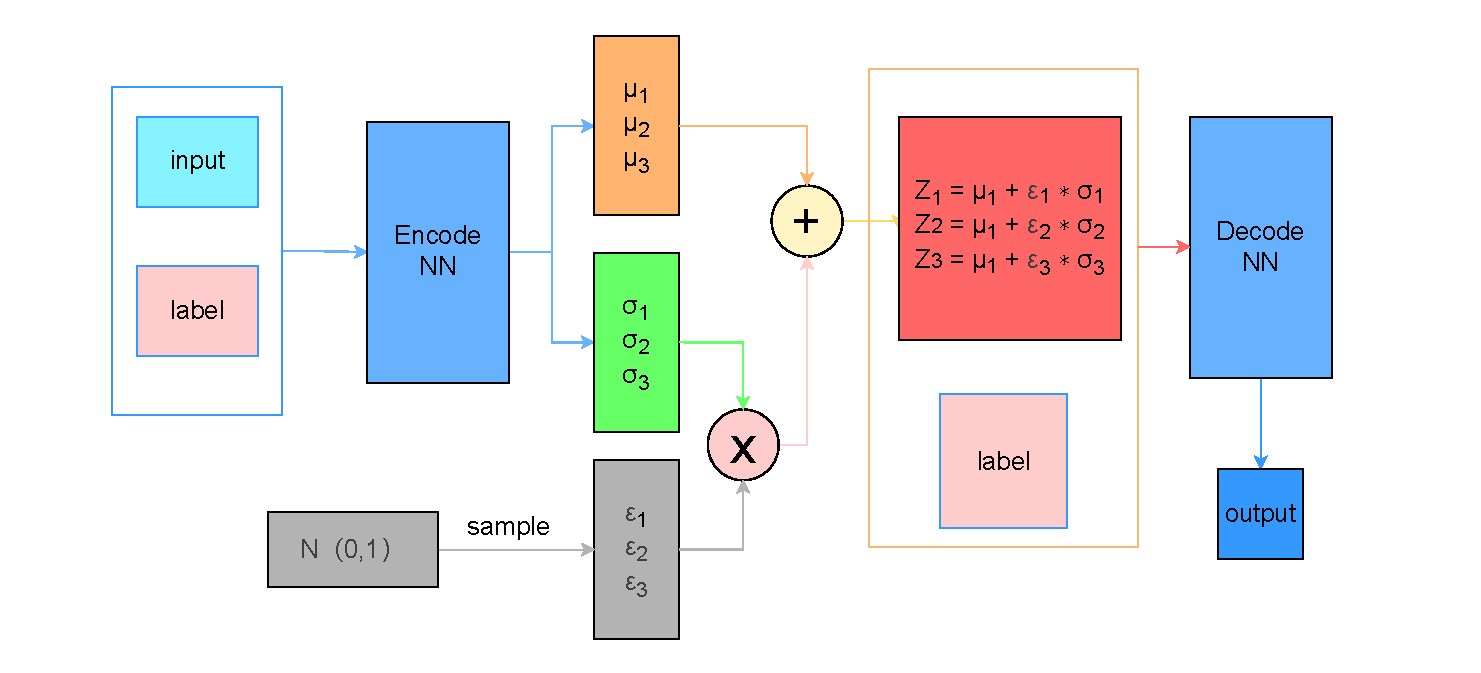
\includegraphics[width=0.8\textwidth]{Fig/CVAE示意图.drawio.pdf}
  \FigureBicaption{\label{cvae illustration}CVAE 示意图}{Schematic illustration of CVAE}
\end{figure}
\begin{equation}
  \mathcal{L}(\theta_E, \theta_D) = \mathbb{E}_{q_{\theta_E}(z|x,y)} \left[ \log p_{\theta_D}(x|z,y) \right] - D_{KL}(q_{\theta_E}(z|x,y) \| p(z|y))
  \label{eq:cvae}
\end{equation}
其中,第一项是重构损失,用于衡量模型输出与真实数据的差异;第二项是 KL散度,用于衡量后验分布与先验分布之间的差异。通过最小化这一损失函数,CVAE能够学习到数据的生成分布,并生成与训练数据类似的样本。
CVAE引入条件变量$y$使得模型能够根据特定条件生成样本,这对于许多实际应用非常重要。例如,在图像生成任务中,条件变量可以控制生成图像的类别或属性。通过指定不同的条件变量,CVAE可以生成不同类别的图像,如不同类型的动物、不同的场景等。这使得CVAE在图像生成领域具有广泛的应用前景。

在自然语言处理任务中,条件变量可以控制生成文本的主题或风格。通过指定不同的条件变量,CVAE可以生成不同主题的文本,如新闻报道、故事、诗歌等。此外,条件变量还可以控制文本的风格,如正式、幽默、悲伤等。这使得 CVAE在自然语言生成领域具有重要的应用价值。

此外,CVAE 还可以在标签数据稀缺的情况下,利用无标签数据学习数据的潜在结构,从而增强模型的泛化能力。在实际应用中,标签数据往往非常稀缺,而无标签数据相对丰富。CVAE可以利用无标签数据学习数据的潜在结构,从而提高模型的性能。这使得CVAE在半监督学习和无监督学习中具有重要的应用价值。

在本文的工作中,我们希望通过已有的流变学性质参数,如特定频率下的储存模量(G')、损耗模量(G")和损耗角正切(tan$\delta$)等,来预测特定的制备参数。CVAE能够将输入数据映射到高维潜在空间,并通过将流变学参数作为条件($y$)输入,生成特定的制备参数。

与传统的深度神经网络(DNN),尤其是回归或分类网络不同,DNN通常直接进行输入到输出的映射,缺乏对潜在空间的建模,因此可能无法捕捉到数据背后复杂的分布。相比之下,CVAE作为生成模型,能够学习输入数据的潜在分布。它不仅依赖于输入数据的特征,还引入了条件信息,使得它能够在潜在空间中生成符合条件的参数,而不仅仅是进行简单的映射。

此外,CVAE通过变分推断捕获数据中的不确定性,能生成多个样本。对于制备参数,可能存在多个合理的组合或生成路径,CVAE通过潜在变量的不同采样来生成这些多样化的样本,从而增强了生成结果的多样性。而传统的DNN模型通常是确定性的,即给定相同的输入总是生成相同的输出,无法有效地表示这种不确定性。

最后,CVAE通过引入变分推断,平衡了重建误差和潜在变量的KL散度,从而在优化过程中不仅考虑了生成结果的质量,还保证了潜在空间的结构化。这使得CVAE能够生成接近原始数据的样本,并通过潜在空间的结构化生成有意义的样本。相比之下,DNN训练时通常只关注误差最小化,缺少对潜在空间结构的显式建模。
\subsection{其他生成式模型}
生成式模型(Generative Models)是机器学习领域的重要研究方向,旨在学习数据的分布特征,从而生成与原始数据相似的新样本。除了变分自编码器(VAE)和条件变分自编码器(CVAE)之外,还有多种生成式模型在不同领域取得了显著成果。

自回归模型基于条件概率链式分解对数据进行建模,通过逐步生成数据单元完成整体构建\cite{bengio2003adaptive}。这类模型在密度估计方面展现出卓越性能,典型代表如PixelCNN和PixelSNAIL已成功应用于图像生成、语音合成等领域。然而其固有特性也带来若干限制:采样过程必须严格遵循序列生成路径,导致高维数据生成效率显著降低;同时模型强制要求将输入数据线性化为固定顺序,这在文本和音频等具有自然时序结构的模态中尚可适用,但对于图像等空间数据而言,最优排列方式的确定缺乏明确依据,且不同的顺序选择可能通过神经网络架构的归纳偏置对最终效果产生潜在影响\cite{bondtaylor2022deep}。

生成对抗网络(Generative Adversarial Networks,GAN)是一种基于博弈论框架的生成模型,其核心由生成器(Generator)与判别器(Discriminator)构成动态博弈系统\cite{NIPS2014_5ca3e9b1}。生成器通过参数化映射函数将潜在空间向量转化为合成数据,旨在捕捉真实数据分布的统计特性;判别器则作为二元分类器,通过迭代优化提升对真实数据与生成数据的鉴别能力。二者在对抗性训练过程中形成"最小-最大"博弈关系:生成器试图生成以假乱真的样本来欺骗判别器,而判别器则持续升级其辨别能力以识别生成样本的统计缺陷,最终推动系统向纳什均衡收敛。相较于传统生成模型,GAN的突出优势在于其能通过对抗机制隐式学习复杂数据分布,生成具有高度视觉保真度的样本(如图像、视频)\cite{Goodfellow2020Generative}。

扩散模型是新一代生成式人工智能的核心范式,其创新性地将数据生成过程建模为物理学启发的渐进式去噪机制\cite{ho2020denoising}。该模型通过构建马尔可夫链,系统性地模拟两个互逆过程:前向扩散阶段将原始数据通过逐步添加高斯噪声退化为随机噪声,反向生成阶段则通过参数化的神经网络学习逆向扩散轨迹,从纯噪声出发通过连续的去噪操作重建出目标数据分布。这种基于随机微分方程(SDE)或概率流常微分方程(ODE)的数学框架,使得模型能够通过变分推断精确优化对数似然下界\cite{song2020score}。相较于GAN,其生成过程具有可解释的物理意义,通过调节去噪步长可实现生成质量与速度的灵活平衡;无需对抗训练避免了模式崩溃风险,确保生成样本的多样性,且理论框架的严密性支持精确的概率密度估计\cite{Cao2024Survey}。
\section{本章小结}
本章围绕深度学习与物理建模的融合框架展开系统性论述,为流变学本构方程的数据驱动建模奠定了坚实的理论基础与技术体系。

在时序建模层面,系统解析了循环神经网络及其衍生架构的时序建模机理,重点探讨了门控循环单元(GRU)在流变学本构时序响应建模中的适用性与局限性,阐明其在处理材料非线性记忆效应(如应力松弛、触变恢复)中的优势及梯度稳定性问题。针对物理约束嵌入方法,深入剖析了物理信息神经网络(PINN)的数学基础与实现范式,为后续构建具有物理一致性的流变学代理模型提供理论支撑。在特征融合方面,通过对比分析多尺度数据整合策略,揭示了注意力机制在动态协调流变实验多源异构数据中的核心价值,为解决复杂流变行为的特征解耦问题开辟新途径。针对生成式建模技术,综述了变分自编码器的概率框架与条件扩展形式。

本研究通过算法体系的多维度解析,为突破传统唯象模型的表征瓶颈、后续构建发展"数据-物理"双驱动的智能本构建模范式提供了理论架构与方法论指导。